\section{Task 1: Model for Tourism Industry in Juneau}

\subsection{Introduction}


In this section we need to select factors to quantify and track the tourism industry in Juneau. 
It is impossible and unnecessary to consider all the factors that may affect the 
tourism industry, only those that are relevant to the problem need to be considered.
Drawing on the idea of the divide-and-conquer algorithm, we first divide the factors 
into three categories: economy, environment and society (aka hidden cost factors). 
The untimate goal is listed below:


\begin{equation}
    \mathcal{F}=(\alpha \cdot \text { Economy }-\beta \cdot \text { Environment }) / \text { Hidden Cost Factors }
\end{equation}

where $\alpha$ and $\beta$ are the weights of the economy and environment, denoting the importance we attach to each category.
Economy means the income generated by the tourism industry, environment means the environmental cost of the tourism industry, and 
society is an indicator that quantifies the satisfaction of the local residents towards the tourism industry.

Our goal is to maximize the final output $\mathcal{F}$. Intuitively, it 
is equivalent to maximizing economy income, minimizing the environmental 
impact and elevating the final scores of hidden cost factors.

Each category is further divided into several minor factors such as local population, 
number of tourists to extrapolate a mathematical model fitting the circumstances in Juneau,
which will be discussed in the following sections.





\subsection{Economy}

In this section we consider the actions that will contribute to the income of the tourism industry in Juneau, which are
tourists' consumption, tax income and fines.

\subsubsection{Tourists' Consumption}

We first calculate the average consumption of tourists in Juneau per day. Since there is no existing official data available, 
we can infer it by other means. According to [5], avearge tax income from tourists in Juneau is 27.7 million dollars in 2018
with a tax rate of 12\%. We can use this information to estimate the average consumption of tourists in Juneau per day according to 
the following equation.

\begin{equation}
    \text{Average Consumption} = \frac{\text{Tax Income}}{\text{Tax Rate} \times \text{Number of Tourists}}
\end{equation}

The number of tourists can be found in Table 2. The average consumption of 
tourists in Juneau per day is calculated as follows:

\begin{equation}
    \text{Average Consumption} = \frac{27.7 \times 10^6}{0.12 \times 1151 \times 10^3} \approx 200.55
\end{equation}

Therefore the function of tourists' consumption regarding the number of tourists is:


\begin{equation}
    \text{Tourists' Consumption} = 200.55 N
\end{equation}

Given that an average of 3 days are spent by each visitor to Juneau, 
the total consumption of tourists should multiply by another 3.

\subsubsection{Tax Income}

According to the official website of Juneau, the tax rate of the tourism industry is 12\%.
The tax income can be calculated as follows:

\begin{equation}
    \text{Tax Income} = 0.12 \times \text{Tourists' Consumption} \approx 24 N
\end{equation}

We should also consider the case when the tax rate is not fixed to propose suggestions to the
government on how to adjust the tax rate to maximize the income of the tourism industry. We
use the data calculated as above as the base case and assume that the tax rate $\eta$ is associated with the number of tourists.

The actual visitors $N$ is calculated as follows:


\begin{equation*}
    N= N_0 \cdot f(\eta)
\end{equation*}

Intuitively, $\eta$ should be negatively correlated with the number of tourists. When $eta$ is 
set to 0, we assume that the number of tourists will be $1.5N_0$, and when $\eta$ is set to 1, the number of tourists will be 0.
Specifically, when $\eta$ is set to the current tax rate 0.12, the number of tourists will be $N_0$. 
Also, $f(\eta)$ should be monotonically decreasing and fall steeply in the range of $[0,0.12]$ and $[0.85,1]$, 
Using the above data
we propose a model that fits the relationship between the tax rate and the number of tourists as follows:

\begin{equation*}
    f(\eta) = -5.5 \eta^3 + 9.1903 \eta^2 - 5.1903 \eta + 1.5, \quad 0 \leq \eta \leq 1
\end{equation*}

Therefore the tax income can be calculated as follows:

\begin{equation}
    \text{Tax Income} = 200.55N \cdot f(\eta), \quad 0 \leq \eta \leq 1
\end{equation}

\subsubsection{Fines}

As there is no official data available, we assume that the 
fine rate is negatively correlated with the amount of fines 
and follows an exponential distribution $f(x) = \lambda \cdot e^{-\lambda x}$. We also assume that 
fined rate falls to 5\% when the amount of fines climbs to 15 dollars, that is:

\begin{equation*}
    \int_0^{15} \lambda \cdot e^{-\lambda x} d x=1-95 \% \Rightarrow \lambda \approx 0.2
\end{equation*}

Therefore the total amount of fines can be calculated as follows:

\begin{equation}
    \text { Fines }=N Q \cdot\left(1-\int_0^Q 0.2 \cdot e^{-0.2 x} d x\right)=N Q \cdot e^{-0.2 Q}
\end{equation}




\subsection{Environment}

% According to the official website of Juneau, its tourism industry is 
% mainly comprised of glacier tours, whale watching, rainforest tours and others.
% We assume each of these activities accounts for a certain percentage of the total environmental impact,
% denoted as $v_1$, $v_2$, $v_3$ and $v_4$ respectively. Due to the receding of glaciers,
% our goal is to lower the percentage of glacier tours and increase the percentage of other activities.

In this section we propose a new model $KAYA_{tourism}$ derived 
from the KAYA model to quantify the environmental impact of the tourism industry in Juneau.

\subsubsection{KAYA Model}

The original KAYA model is a mathematical model that 
describes the relationship between the total 
amount of CO2 emissions and the four factors 
that affect it: population, GDP per capita, energy intensity and carbon intensity.
 The KAYA model is expressed as follows:

\begin{equation*}
    \text { CO2 Emissions }=P \times GDP \times E I \times C I
\end{equation*}

where $P$ denotes the population, $GDP$ denotes the GDP per capita, 
$EI$ denotes the energy intensity and $CI$ denotes the carbon intensity.
This model falls short when only considering the environmental impact of the tourism industry.
Based on the data we collect and the goal of our project, we propose a new model $KAYA_{tourism}$.


\subsubsection{$KAYA_{Tourism}$ Model}

The $KAYA_{Tourism}$ model is expressed as follows:

\begin{equation}
    CO_{2\_Tourism}=G \times CG_{Tourism}
\end{equation}

where $G$ denotes the gross income of the tourism industry and $CG = EI \times CI$. To calculate 
the emission of $CO_2$ in the tourism industry, we first looked up the data of the Juneau's carbon emission and
GDP across the country and calculated the $CG_{All}$ across the country. $CG_{Tourism}$ can 
be calculated as $CG_{Tourism} = CG_{All} \times Ratio $  where $Ratio$ is the 
ratio tourism accounts for across all industries. The income of the tourism industry in Juneau 
has been calculatd in the previous section, and the $CO_{2\_Tourism}$ can thus be estimated.
It should be noted that $G$ and $CG_{Tourism}$ are both linear functions of the number of tourists $N$,
therefore when fitting and regressing $CO_{2\_Tourism}$ quadratic regression should be used.

Alongside the historical data, future predictions are also conducted using the \textit{SARIMAX} model.
The results are listed below.

\begin{figure}[H]
    \centering
    \begin{minipage}{0.32\textwidth}
        \centering
        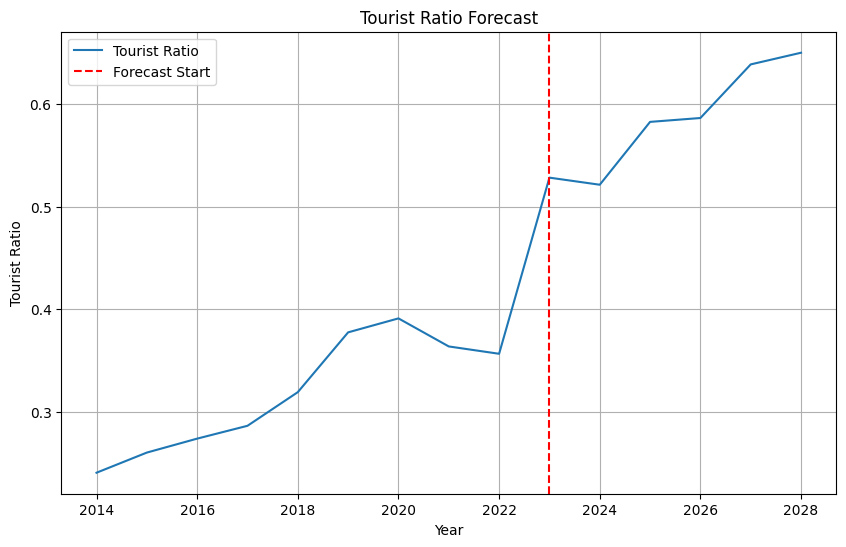
\includegraphics[width=\textwidth]{Ratio.jpg}
        % \caption{Caption 1}
    \end{minipage}
    \begin{minipage}{0.32\textwidth}
        \centering
        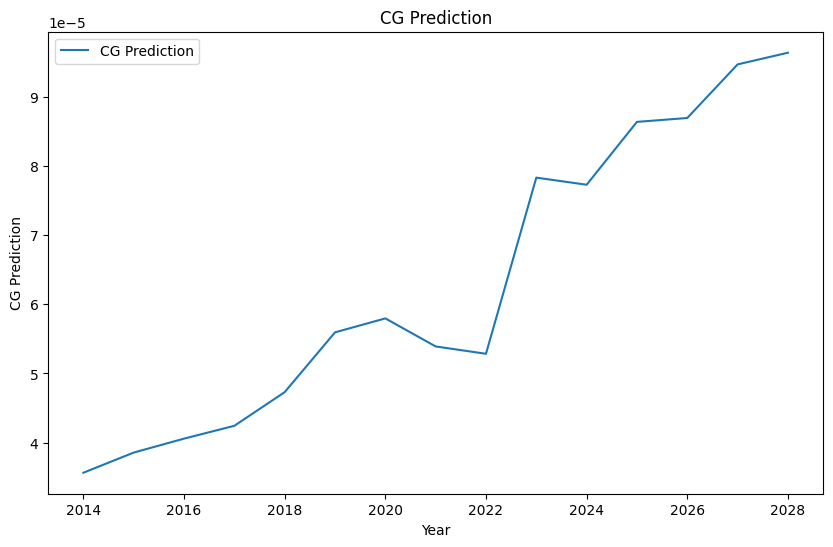
\includegraphics[width=\textwidth]{CG_pred.jpg}
        % \caption{Caption 2}
    \end{minipage}
    \begin{minipage}{0.32\textwidth}
        \centering
        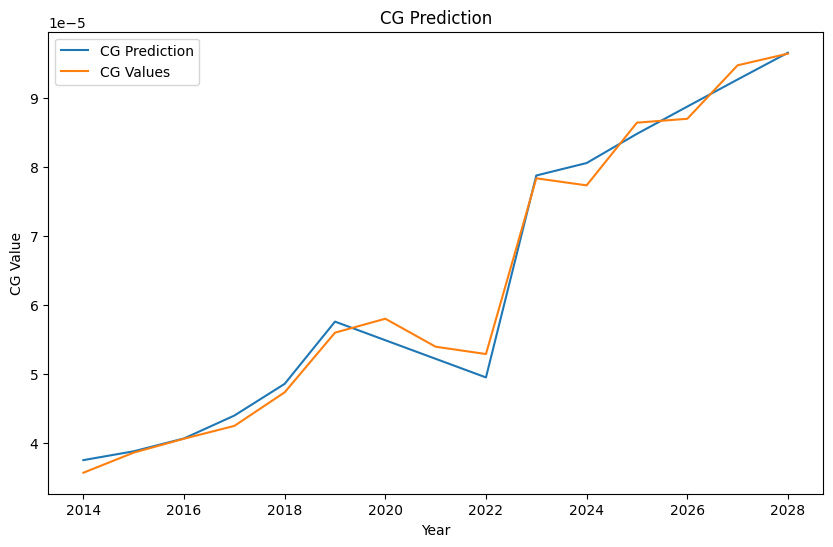
\includegraphics[width=\textwidth]{CG_pred2.jpg}
        % \caption{Caption 3}
    \end{minipage}
\end{figure}

\begin{figure}[H]
    \centering
    \begin{minipage}{0.32\textwidth}
        \centering
        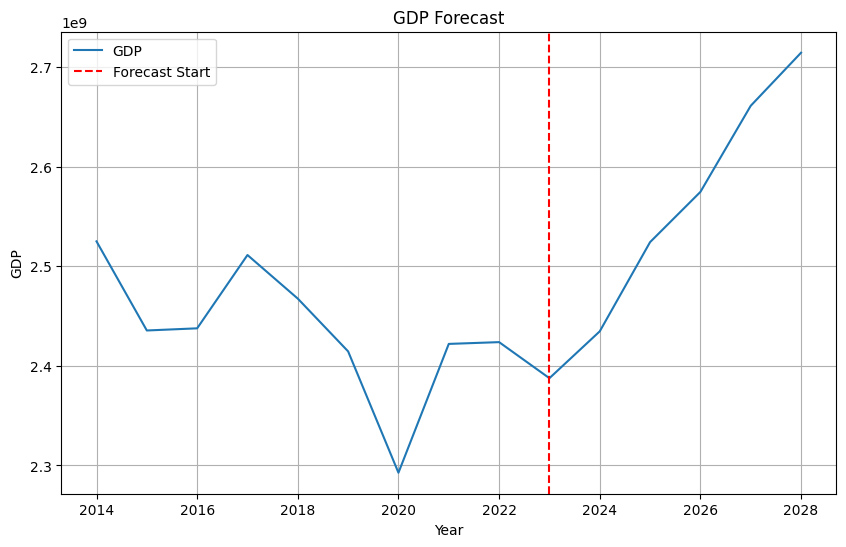
\includegraphics[width=\textwidth]{GDP.jpg}
        % \caption{Caption 4}
    \end{minipage}
    \begin{minipage}{0.32\textwidth}
        \centering
        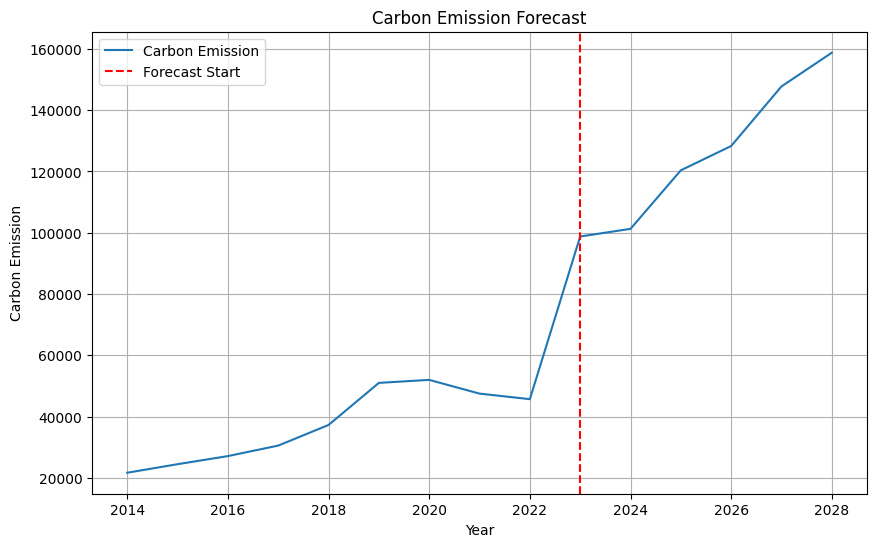
\includegraphics[width=\textwidth]{Emission.jpg}
        % \caption{Caption 5}
    \end{minipage}
    \begin{minipage}{0.32\textwidth}
        \centering
        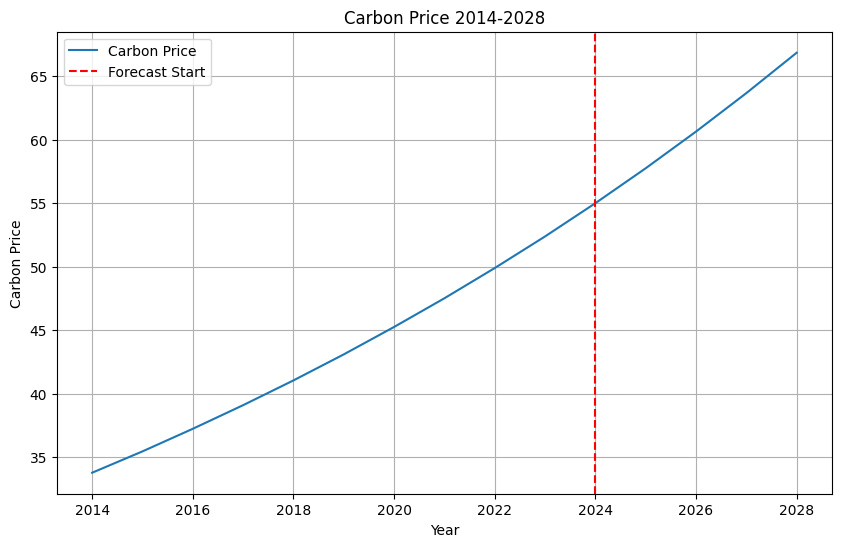
\includegraphics[width=\textwidth]{Price.jpg}
        % \caption{Caption 6}
    \end{minipage}
\end{figure}

\begin{figure}[H]
    \centering
    \begin{minipage}{0.32\textwidth}
        \centering
        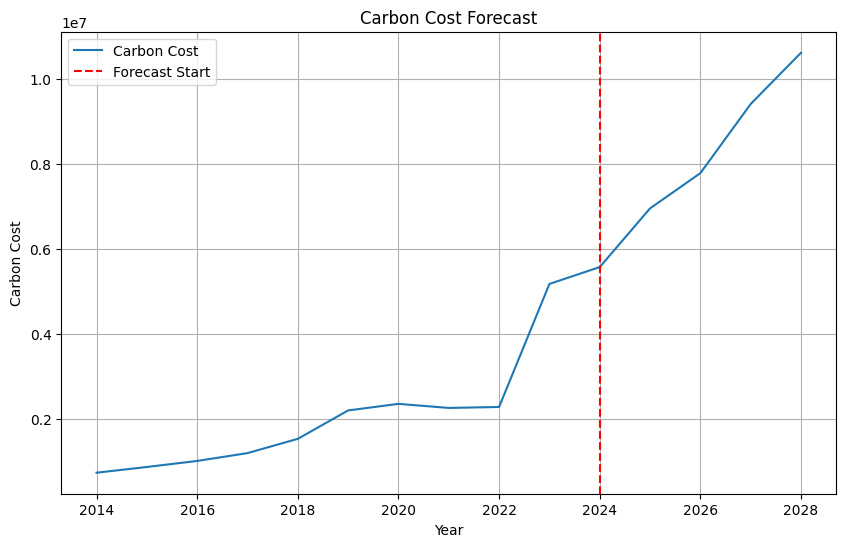
\includegraphics[width=\textwidth]{Cost.jpg}
        % \caption{Caption 7}
    \end{minipage}
    \begin{minipage}{0.32\textwidth}
        \centering
        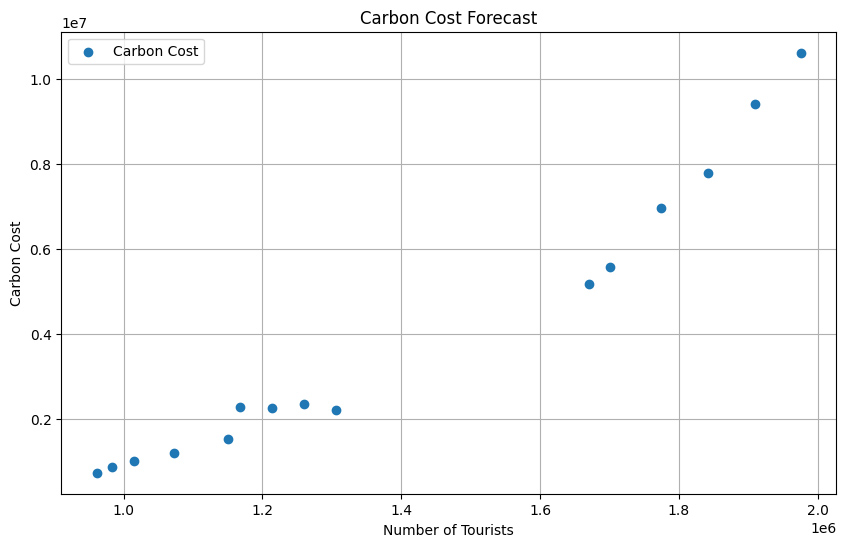
\includegraphics[width=\textwidth]{Carbon_pred1.jpg}
        % \caption{Caption 8}
    \end{minipage}
    \begin{minipage}{0.33\textwidth}
        \centering
        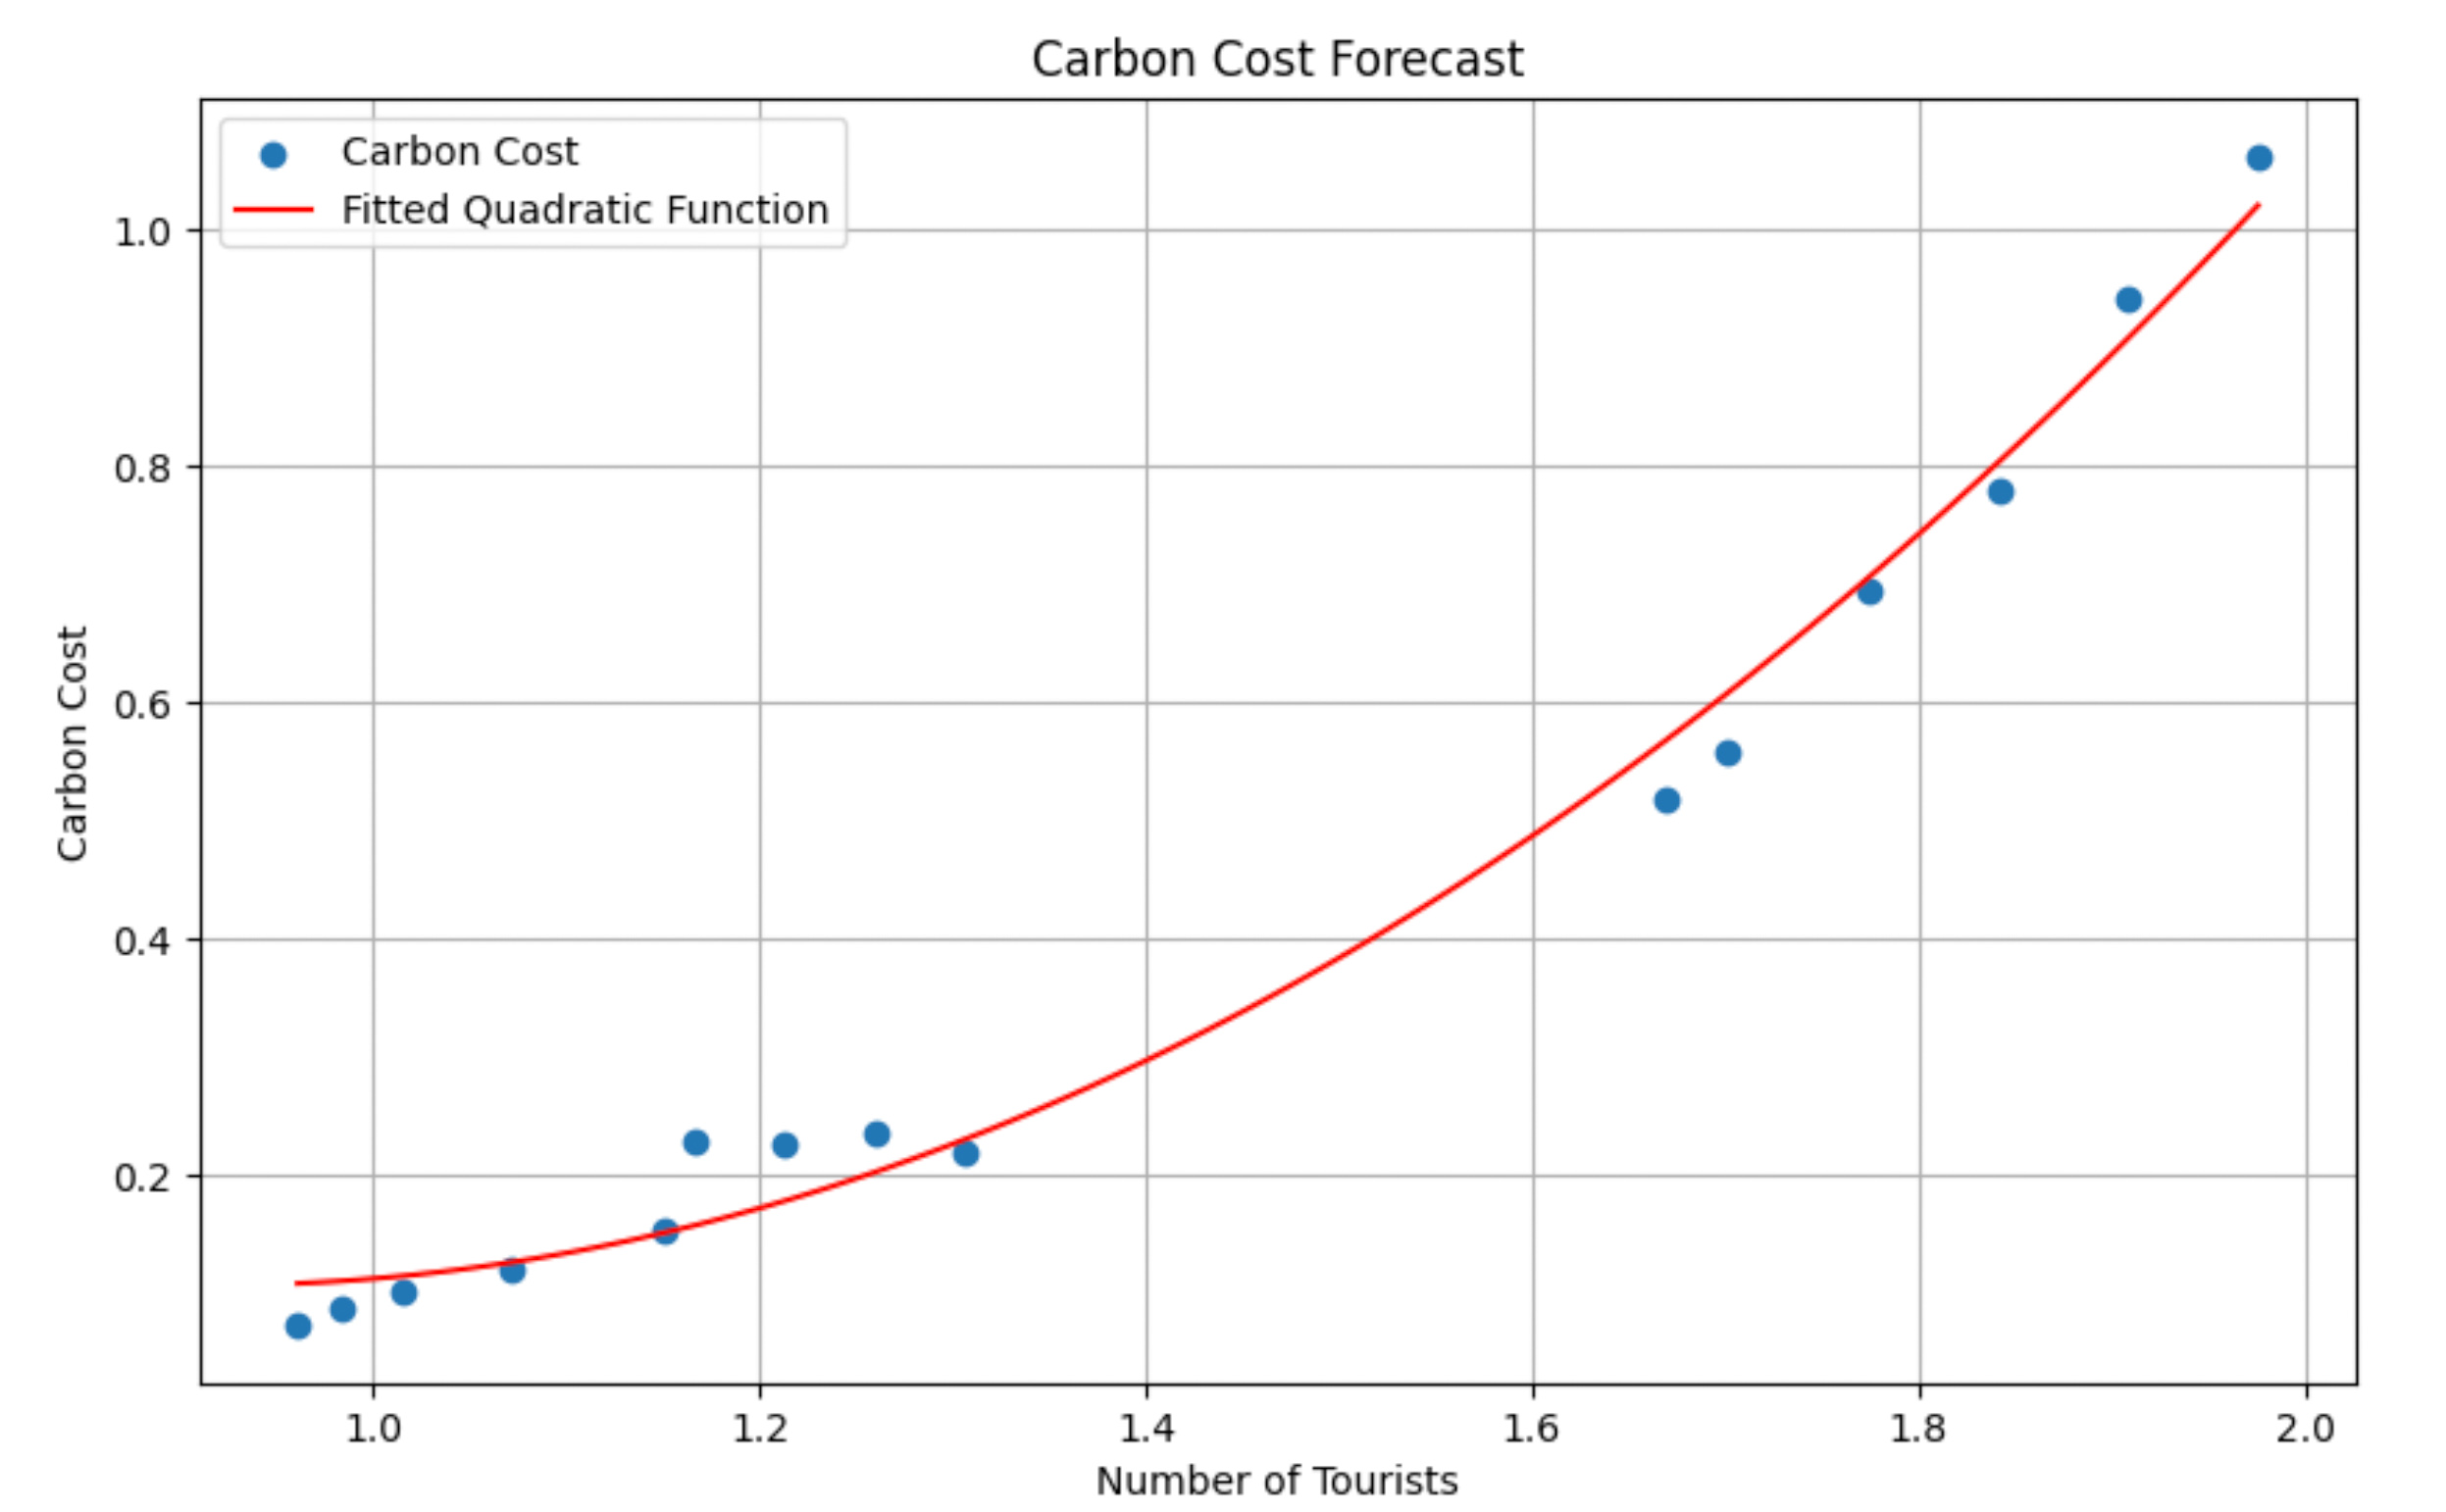
\includegraphics[width=\textwidth]{Carbon_pred2.jpg}
        % \caption{Caption 9}
    \end{minipage}
\end{figure}

From subplot 9 we can see that a quadratic regression 
fits the data well with an $R^2$ value of over 0.99.
The fitting function yields the following results:

\begin{equation}
    CO_{2\_Tourism} = 0.815 \times \frac{N^2}{10^5} - 14.95N+7924000
\end{equation}



\subsection{Hidden Cost Factors}

Societal factors such as infrastructure, price of housing products, and the mental
loss due to the overcrowding and rowdy tourists all account for the hidden costs of the tourism industry.

\subsubsection{Data Processing}

Firstly we collected comprehensive and accurate data from all sources regarding Juneau, including the following factors:

\textit{Satisfy\_Score},\textit{Crowding\_at\_Mendenhall\_Glacier}, \textit{Crowding\_on\_sidewalks\_downtown}, \\ \textit{Vehicle\_congestion\_downtown}, \textit{Flightseeing\_noise}, \textit{Air\_emissions\_from\_cruise\_ships},\\ \textit{Vehicle\_congestion\_outside\_of\_downtown}, 
\textit{Whale\_watching\_boat\_traffic\_and\_wakes}, \textit{Crowding\_on\_trails}, \textit{Street\_Services}, \textit{Wastewater}, \textit{Public\_Transit}, \textit{Parks\_and\_Recreation}, 
\textit{Docks}, \textit{Ports}

We then use the data $N$ and $N_{Local}$ calculated in \textit{Section 3} to fit a linear regression model. The results are as follows:

\begin{figure}[htbp]
    \centering
    \begin{minipage}[t]{0.49\textwidth}
        \centering
        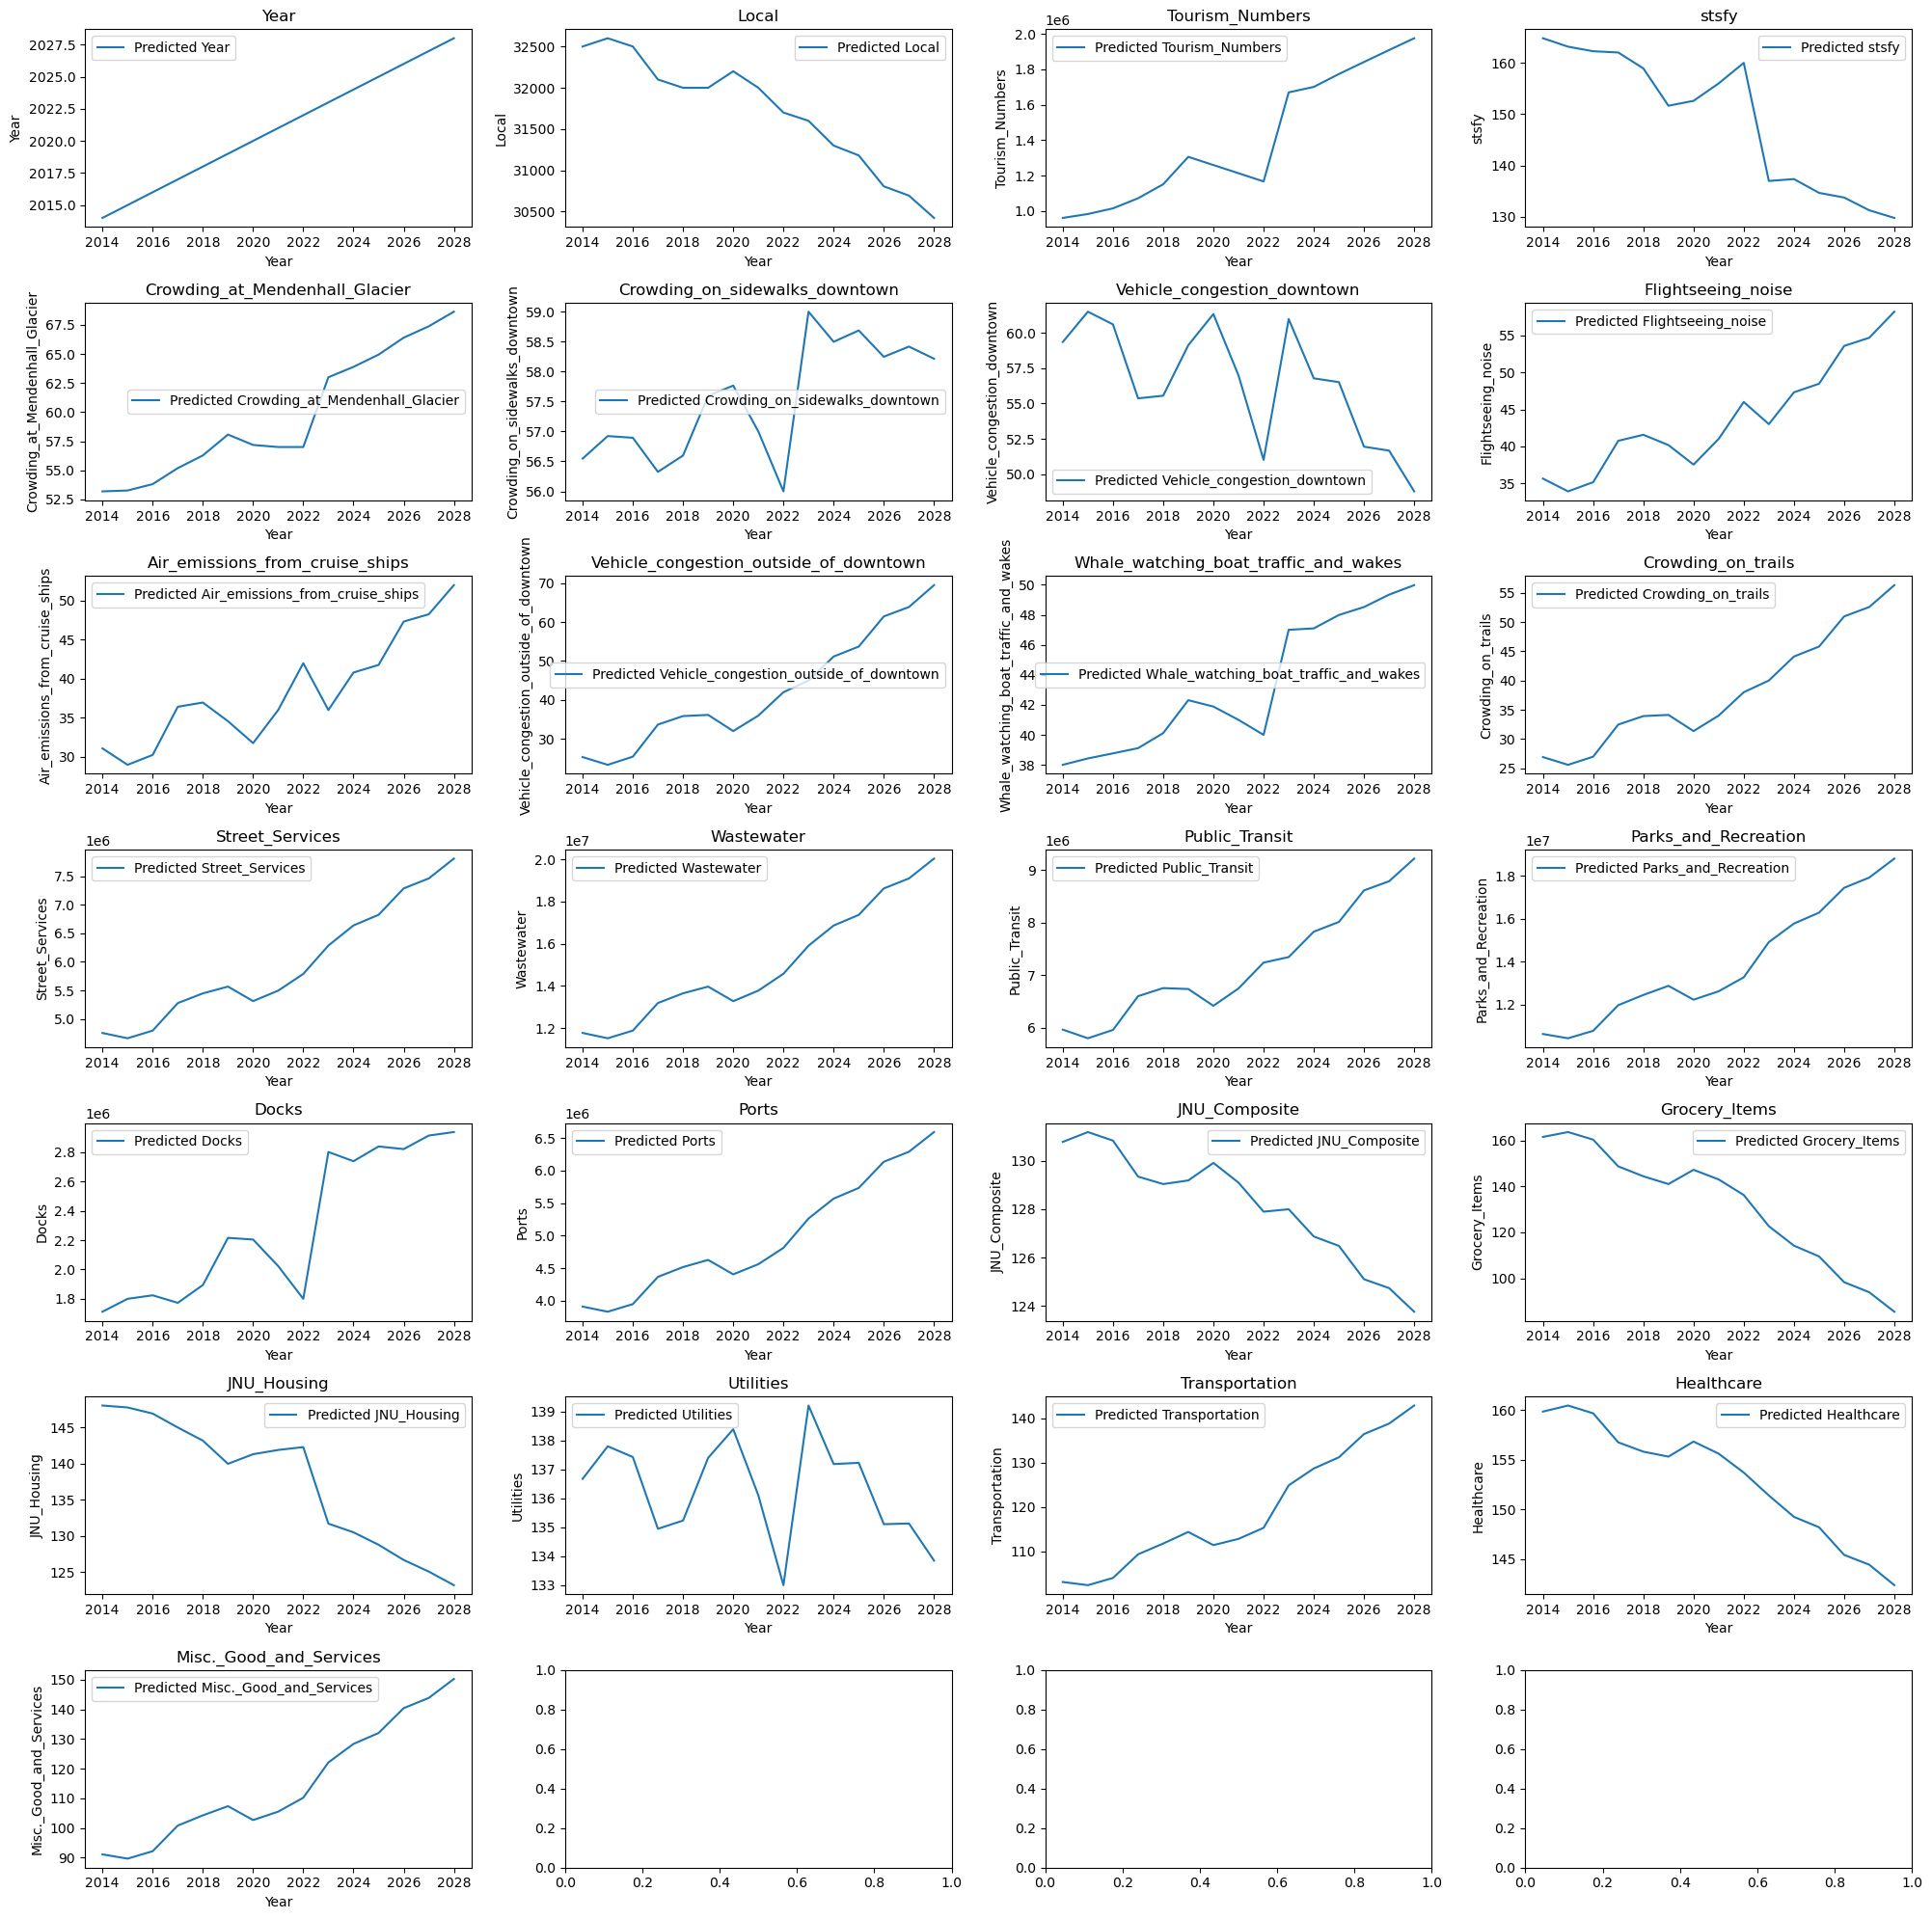
\includegraphics[width=1\textwidth]{2dLinear_1.jpg} % 插入图片
	    %   \vspace{-0.8cm}
        % \caption{}
    \end{minipage}
    \hfill
	%   \hspace{0.1\textwidth} % 调整这里的值来改变两张图片之间的间距
    \begin{minipage}[t]{0.49\textwidth}
        \centering
        \includegraphics[width=1\textwidth]{2dLinear_2.jpg} % 插入图片
	    %   \vspace{-0.8cm}
        % \caption{}
\end{minipage}
\caption{Bivariate Linear Regression}
\end{figure}

Only a fraction of results are shown here. The full results can be found in \textit{Appendix A}.

\textbf{\textit{Model for stsfy: }}

$\text{stsfy} = -4.693528652706527\times 10^{-5} N - 0.0060844912311383 \times N_{local} + 407.6518514$

\textbf{\textit{Model for Crowding\_at\_Mendenhall\_Glacier: }}

$\text{Crowding\_at\_Mendenhall\_Glacier} = 1.1573084349139379\times 10^{-5} N - 0.0017873857238289111 \times N_{local} + 100.15433801$


\subsubsection{Entropy Weight Method}

The Entropy Weight Method (EWM) is a quantitative technique commonly used 
to determine the weight or importance of various factors in multi-criteria 
decision-making. It is based on the concept of information entropy from 
information theory, which measures the degree of disorder or uncertainty in a system.
We mainly utilized the following equations.

\paragraph{Convert to Probability Matrix}


\[P_{i j}=\frac{X_{i j}}{\sum_{i=1}^n X_{i j}}\]


where:
\begin{itemize}
    \item $P_{i j}$ is the probability value of the $i$-th row and $j$-th column.
    \item $X_{i j}$ is the value of the $i$-th row and $j$-th column in the original data matrix.
    \item $\sum_{i=1}^n X_{i j}$ is the sum of all elements in the $j$-th column.
\end{itemize}

\paragraph{Calculate Information Entropy}


\[H_j=-k \sum_{i=1}^n P_{i j} \ln \left(P_{i j}+\epsilon\right)\]

where:

\begin{itemize}
    \item $H_j$ is the entropy value of the $j$-th index.
    \item $k=\frac{1}{\ln (n)}$ is the normalization coefficient to ensure that the entropy value is within the range of $[0,1]$.
    \item $P_{i j}$ is the probability value.
    \item $\epsilon$ is a very small value (e.g. $10^{-12}$) to avoid numerical errors in the logarithm calculation.
\end{itemize}

\vspace{0.5cm}

The calculated results are shown below:

\begin{table}[ht]
    \centering
    \renewcommand{\arraystretch}{1.3}
    \caption{Factors and Their Weights}
    \begin{tabular}{|l|c|l|c|}
    \hline
    \textbf{Factor} & \textbf{Weight} & \textbf{Factor} & \textbf{Weight} \\ \hline
    stsfy & 0.029112 & Wastewater & 0.038384 \\ \hline
    Crowding at Mendenhall Glacier & 0.029089 & Public Transit & 0.012025 \\ \hline
    Crowding on sidewalks downtown & 0.002553 & Parks and Recreation & 0.180182 \\ \hline
    Vehicle congestion downtown & 0.058313 & Docks & 0.024321 \\ \hline
    Flightseeing noise & 0.025751 & Ports & 0.121009 \\ \hline
    Air emissions from cruise ships & 0.139424 & Grocery Items & 0.015780 \\ \hline
    Vehicle congestion outside of downtown & 0.129145 & JNU Housing & 0.034101 \\ \hline
    Whale watching boat traffic and wakes & 0.021685 & Utilities & 0.002685 \\ \hline
    Crowding on trails & 0.034678 & Transportation & 0.034639 \\ \hline
    Street Services & 0.067125 & & \\ \hline
    \end{tabular}
    \end{table}

It can be noted that \textit{Air emissions from cruise ships} and \textit{Vehicle congestion outside of downtown} are the two important factors that affect the hidden cost of the tourism industry in Juneau, 
which denotes that our model is able to capture the essence of the problem and the need of people. It also provides a comprehensive and accurate solution.
    

\subsubsection{Social Impact Model}

Multiplying the weight of each factor by the corresponding value and summing them up, we can get the social impact $\mathcal{I}$.
The result yields:

\begin{equation}
    \mathcal{I}=5.011\times 10^{-9} N -0.002 \times N_{Local}+69.93
\end{equation}


\subsection{Summary}



Summing up all the three categories, we can get the final output of the model:

\begin{equation}
    \begin{aligned}
    &\left\{\begin{array}{l}
    \mathcal{F}=(\alpha \cdot \text { Economy }-\beta \cdot \text { Environment }) / \text { Society } \\[10pt]
    \text { Economy }=200.55 N \cdot f(\eta) \cdot (\eta+1)+NQ\cdot e^{-0.2 Q} \\[10pt]
    \text { Environment }=0.815 \cdot \frac{N^2}{10^5}-14.95 N+7924000 \\[10pt]
    \text { Society }=5.011\times 10^{-9} N -0.002 \times N_{Local}+69.93 \\[10pt]
    f(\eta)=-5.5 \eta^3+9.1903 \eta^2-5.1903 \eta+1.5, \quad 0 \leq \eta \leq 1
    \end{array}\right.
    \end{aligned}
\end{equation}

where $N,Q,\eta$ are independent variables, $\alpha$, $\beta$ 
and are parameters that can be adjusted accordingly, 
$N_{Local}$ is the local population of Juneau assumed fixed.
Our goal is to find the optimal value of $N,Q,\eta$ that maximizes the output $\mathcal{F}$.

Since the number of tourists in the coming year is related to the number of tourists in the previous year, 
we use the $N$ in 2024 to predict the parameters in 2025, and the results are shown below.

When $\alpha$ is set to 1 and $\beta$ is set to 30, 
the optimal value of $N,Q,\eta$ is calculated as follows:

\begin{equation}
    \begin{aligned}
    &\left\{\begin{array}{l}
    N_{Max} = 1408 \\[10pt]
    N=1264 \\[10pt]
    Q=5 \\[10pt]
    \eta=0.221
    \end{array}\right.
    \end{aligned}
\end{equation}

The results suggest a feasible and effective strategy that the government can implement to promote sustainable development. 

The proposed measures include reducing the maximum tourist capacity from 1.728 million in 2024 to 1.408 million, increasing the tax rate to 0.221, and introducing a 5\$ environmental penalty. 

This strategy not only alleviates the pressure on Juneau's local ecosystem but also reduces the strain on essential infrastructure, such as water supply and public transportation. Additionally, it contributes to enhancing the overall well-being and satisfaction of local residents.

\subsection{Sensitivity Analysis}

To evaluate the robustness of our model, we conduct a sensitivity analysis.
Since there isn't many factors that can be adjusted, we don't need to use the Principal Component Analysis (PCA).

The results are shown below:

\begin{figure}[H]
    \centering
    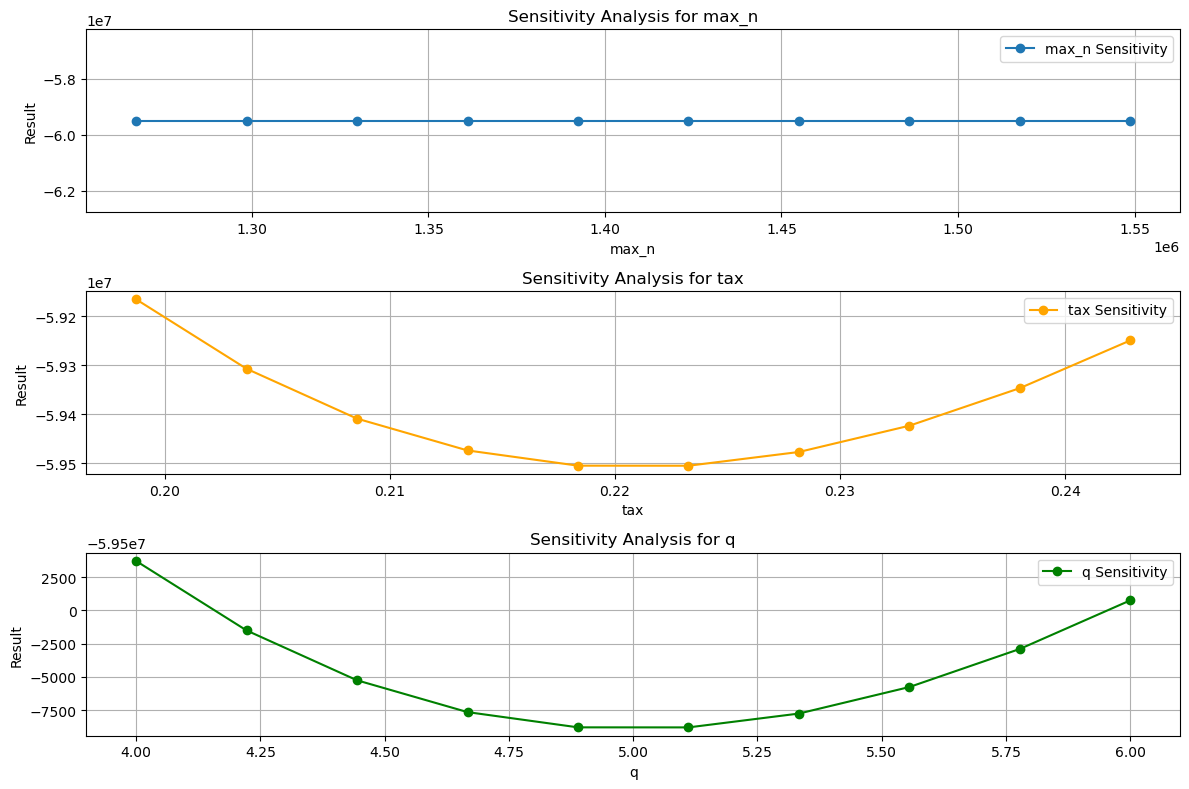
\includegraphics[width=0.97\textwidth]{Sensitivity_Analysis.png} % 插入图片
    \vspace{-0.3cm}
    \caption{Sensitivity Analysis}
\end{figure}

It can be noted that when $\eta$ (tax rate) and $q$ are held constant, 
the output $\mathcal{F}$ does not change significantly with the change of $N_{Max}$.
However, when $\eta$ becomes the independent variable, the output $\mathcal{F}$
budges significantly with the change of $\eta$. The result is similar when $q$ (fine amount) becomes the independent variable.
Therefore, we can conclude that $N_{Max}$ has minimal impact on the result, 
$\eta$ shows moderate sensitivity with a non-linear effect, 
and $q$ is the most sensitive, displaying significant influence on 
the output within its range.